\documentclass[journal,a4paper]{IEEEtran}

% some very useful LaTeX packages include:
%\usepackage{cite}      
\usepackage{graphicx}   
%\usepackage{subfigure} 
\usepackage{url}       
\usepackage{amsmath}    
\usepackage{caption2}
% Your document starts here!
\begin{document}

% Define document title and author
	\title{Weekly Report}
	\author{Adviser: Prof. Yang Wen \\Student: Cheng Wensheng\\ Period: 2018.3.5- 3.11
	}
	\markboth{Visual Information Processing Group}{}
	\maketitle

% Write abstract here
\begin{abstract}
	This week I mainly put my effort on preparing the data set and training DeepLab V2 model with this.
\end{abstract}

% Each section begins with a \section{title} command
\section{Data Set}
	% \PARstart{}{} creates a tall first letter for this first paragraph
	\PARstart{T}{he} original data set the author used is Pascal VOC 2012. So we need to train it on our data set.
	\begin{itemize}
		\item We searched many related papers for proper data set. However, there are no visible spectral remote sensing data set we desired. So I have to build our own data set. 
		\item We tried Google Maps, and attempted to remove text labels and extract 4 targets, including forest, road, building and river. But for Google Maps, I can't separate \textbf{building} from other objects, since there is only one button to control \textbf{man made}, which contains building and other man-made objects. 
		\item \textbf{Solution:} Finally, I found one useful website called \textbf{Mapbox}. It fulfills our requirements perfectly, although it limits the number of images downloaded to 5 per account. The satellite image is Fig.~\ref{fig:sat}, the label image is Fig.~\ref{fig:label}.
	\end{itemize}

% Main Part
\section{Training}
	% LaTeX takes complete care of your document layout ...
	After converting data set to the same format with the original one, we started training the model with our data set. During the procedure, we found that on training set, the accuracy can achieve \textbf{80\%}. But on testing set, it's only about \textbf{60\%}, which is really low. We plan to try following measures to improve performance.
	\begin{itemize}
		\item \textbf{Extend data set.} We have $1\,000$ images with size of 350$\times$350 at first. I plan to download more images from \textbf{Mapbox} to train another.
		\item \textbf{Hyperparameters.} Since there is a bunch of parameters, I will try to adjust them to see the result. 
	\end{itemize}

	\begin{figure}[!hbt]
		% Center the figure.
		\begin{center}
		% Include the eps file, scale it such that it's width equals the column width. You can also put width=8cm for example...
%		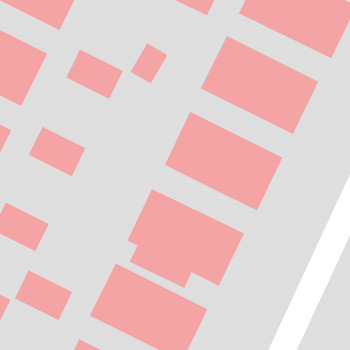
\includegraphics[width=\columnwidth]{LAB01-00002}
		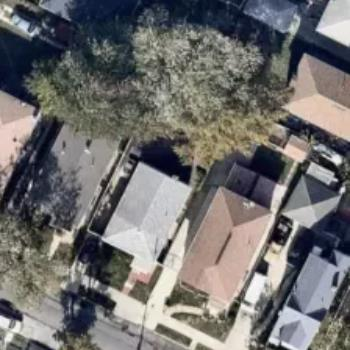
\includegraphics[width=\columnwidth]{SAT01-00000}
		% Create a subtitle for the figure.
		\caption{Satellite image}
		% Define the label of the figure. It's good to use 'fig:title', so you know that the label belongs to a figure.
		\label{fig:sat}
		\end{center}
	\end{figure}

	\begin{figure}[!hbt]
	% Center the figure.
	\vspace{-1cm}
		\begin{center}
		% Include the eps file, scale it such that it's width equals the column width. You can also put width=8cm for example...
		%		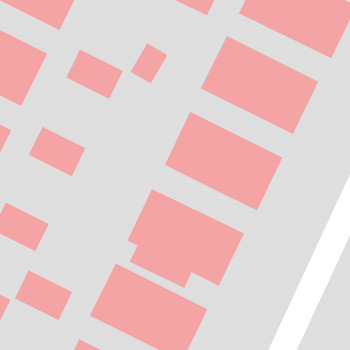
\includegraphics[width=\columnwidth]{LAB01-00002}
		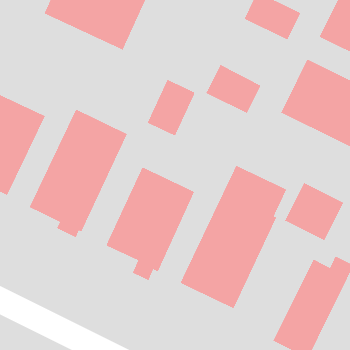
\includegraphics[width=\columnwidth]{LAB01-00000}
		% Create a subtitle for the figure.
		\caption{Label image}
		% Define the label of the figure. It's good to use 'fig:title', so you know that the label belongs to a figure.
		\label{fig:label}
		\end{center}
	\end{figure}	


% Now we need a bibliography:
%\begin{thebibliography}{5}
%
%	%Each item starts with a \bibitem{reference} command and the details thereafter.
%	\bibitem{HOP96} % Transaction paper
%	J.~Hagenauer, E.~Offer, and L.~Papke. Iterative decoding of binary block
%	and convolutional codes. {\em IEEE Trans. Inform. Theory},
%	vol.~42, no.~2, pp.~429–-445, Mar. 1996.
%
%	\bibitem{MJH06} % Conference paper
%	T.~Mayer, H.~Jenkac, and J.~Hagenauer. Turbo base-station cooperation for intercell interference cancellation. {\em IEEE Int. Conf. Commun. (ICC)}, Istanbul, Turkey, pp.~356--361, June 2006.
%
%	\bibitem{Proakis} % Book
%	J.~G.~Proakis. {\em Digital Communications}. McGraw-Hill Book Co.,
%	New York, USA, 3rd edition, 1995.
%
%	\bibitem{talk} % Web document
%	F.~R.~Kschischang. Giving a talk: Guidelines for the Preparation and Presentation of Technical Seminars.
%	\url{http://www.comm.toronto.edu/frank/guide/guide.pdf}.
%
%	\bibitem{5}
%	IEEE Transactions \LaTeX and Microsoft Word Style Files.
%	\url{http://www.ieee.org/web/publications/authors/transjnl/index.html}
%
%\end{thebibliography}

% Your document ends here!
\end{document}